% CVPR 2026 Paper Template; see https://github.com/cvpr-org/author-kit

\documentclass[10pt,twocolumn,letterpaper]{article}

%%%%%%%%% PAPER TYPE
% Camera-ready style with page numbers. NOTE: do not switch to [review]:
% review mode anonymizes the author block, and the assignment requires the
% team members' names on the cover page.
\usepackage[pagenumbers]{cvpr}

% Import additional packages in the preamble file, before hyperref
%% This file contains a number of tweaks that are typically applied to the main document.
%% They are not enabled by default, but can be enabled by uncommenting the relevant lines.

%%
%% Packages used by this report that cvpr.sty does not already load
%%
\usepackage{multirow}

%%
%% Inline annotations; for predefined colors, refer to "dvipsnames" in the xcolor package:
%% https://tinyurl.com/overleaf-colors
%%
\newcommand{\red}[1]{{\color{red}#1}}
\newcommand{\todo}[1]{{\color{red}#1}}
\newcommand{\TODO}[1]{\textbf{\color{red}[TODO: #1]}}
%%
%% disable for camera ready / submission by uncommenting these lines  
%%
% \renewcommand{\TODO}[1]{}
% \renewcommand{\todo}[1]{#1}

%%
%% work harder in optimizing text layout. Typically shrinks text by 1/6 of page, enable
%% it at the very end of the writing process, when you are just above the page limit
%%
\usepackage{microtype}

%%
%% fine-tune paragraph spacing
%%
% \renewcommand{\paragraph}[1]{\vspace{.5em}\noindent\textbf{#1.}}

%%
%% globally adjusts space between figure and caption
%%
% \setlength{\abovecaptionskip}{.5em}


%%
%% Allows "the use of \paper to refer to the project name"
%% with automatic management of space at the end of the word
%%
% \usepackage{xspace}
% \newcommand{\paper}{ProjectName\xspace}

%%
%% Commonly used math definitions
%%
% \DeclareMathOperator*{\argmin}{arg\,min}
% \DeclareMathOperator*{\argmax}{arg\,max}

%%
%% Tigthen underline
%%
% \usepackage{soul}
% \setuldepth{foobar}

% Figures live alongside this file; the parent fallback also finds the copies the
% notebooks write into midterm/ if the local ones are ever removed.
\graphicspath{{./}{../}}

\definecolor{cvprblue}{rgb}{0.21,0.49,0.74}
\usepackage[pagebackref,breaklinks,colorlinks,allcolors=cvprblue]{hyperref}

%%%%%%%%% PAPER ID
\def\paperID{*****}
\def\confName{CVPR}
\def\confYear{2026}

%%%%%%%%% TITLE
\title{Semi-Supervised Stopping-Reason Labeling and Phase-Aware Outcome\\
Prediction for Clinical Trials\\
\vspace{0.35em}
\large CS5785 / ORIE5750 / ECE5414 --- Midterm Project}

%%%%%%%%% AUTHORS
\author{Anirudha Hadagali\\
Cornell University
\and
Michael Mazzola\\
Cornell University
\and
Tarun Mandalapu\\
Cornell University
}

\begin{document}
\maketitle

\begin{abstract}
We study semi-supervised learning on a clinical-trial corpus in which only 157 of
1,171 training trials carry stopping-reason labels. \textbf{Part~1} predicts five
binary stopping reasons (Safety, Funding, Efficacy, Recruitment, Other) from 150-d
reason embeddings. Our final model couples an unsupervised diagonal-covariance
Gaussian mixture (30 components, fit on all 1,561 trials without labels) to a
class-balanced multinomial logistic regression blended with a cosine $k$NN, and
uses the mixture posterior as a prior inside two rounds of confidence-thresholded
self-training. It reaches sample-F1 0.893 and macro-F1 0.714 on the validation set
(0.914 / 0.814 under repeated cross-validation) and 0.894 on the Kaggle test set.
An ablation shows that eligibility criteria, disease text, Morgan fingerprints and
start year all fail to improve on the embeddings alone. \textbf{Part~2} predicts
per-phase trial success. A stacked ensemble of eight field-specific base models,
combined by a phase-aware logistic meta-model and trained with exponential recency
weights, cuts mean validation log loss from 0.591 to 0.556 and raises mean PR-AUC
from 0.796 to 0.814 relative to a criteria-only per-phase baseline. Error analysis
keyed on the Part~1 reasons shows that failures concentrate in Phase~III and in
trials with no recorded stopping reason, and that the improved model reduces those
error rates most.
\end{abstract}


\noindent\textbf{Team responsibilities.}
All three authors collaborated on Part~1, Part~2 and this report.
\textbf{Michael Mazzola} led the optimization of the Part~1 reason-labeling
solution. \textbf{Tarun Mandalapu} built the initial Part~2 outcome classifier,
which \textbf{Anirudha Hadagali} then optimized into the final stacked ensemble.
Tarun Mandalapu wrote the report.

\section{Methods}
\label{sec:methods}

\subsection{Part 1: generating the missing reason labels}

\paragraph{Data and features.}
 The Part~1 files, derived from
ClinicalTrials.gov~\cite{clinicaltrials} with some processing performed by course staff, hold 1,561 trials that stopped early: 1,171 training trials of
which only 157 carry visible labels (the remaining 1,014 have all five reasons
masked as $-100$), 78 fully labeled validation trials, and 312 unlabeled test
trials from later start years. Our features are the 150 reason-embedding
dimensions, standardized with a scaler fit on the pooled train, validation and
test embeddings. We attempted feature-set variations including additional trial metadata but found that it performed worse than the model trained only on \texttt{why\_stop} embeddings.

\paragraph{Unsupervised step.}
We reduce the standardized embeddings to 30 principal components and fit a
Gaussian mixture with 30 diagonal-covariance components on all 1,561 trials.
Components are initialized from the default $k$-means++ responsibilities of
\texttt{scikit-learn}~\cite{pedregosa2011scikit}, with 3 restarts and the
best-log-likelihood run kept (\texttt{random\_state}=0).
Expectation--maximization~\cite{dempster1977em} stops once the mean
log-likelihood changes by less than $10^{-3}$ between iterations; the selected run
converged after 30 of the permitted 100 iterations.

Each component is then turned into a reason distribution by a
``cluster-then-label'' step. For a given component, we average the label vectors
of the labeled trials, weighting each trial by how strongly the mixture assigns it
to that component. A trial with two reasons contributes half a count to each, so
every trial carries the same total weight regardless of how many reasons it has.
To that average we add a single pseudo-count of the overall reason distribution,
which keeps components holding few or no labeled trials from collapsing onto a
degenerate estimate and instead pulls them toward the global average. A new trial
is scored by taking its component memberships and averaging the corresponding
component distributions.

\paragraph{Supervised base model.}
The supervised half is a multinomial logistic regression over the five reasons
($C = 0.3$, at most 3000 solver iterations). A multi-label trial is handled by
entering it once for each reason it carries, splitting one unit of weight evenly
between those copies, so a two-reason trial contributes half a count to each
rather than counting twice. Classes are then reweighted so that the rare reasons
are not drowned out by Recruitment, which appears on 64\% of trials. We average
this model's predictions with those of a cosine-similarity nearest-neighbour
classifier, giving the regression 70\% of the weight and the neighbours 30\%. The
neighbour model looks at a trial's 10 closest trials and averages their reasons,
weighting each neighbour by the square of its similarity so that close matches
count for much more than distant ones. This average of the two is what we call the
base model.

\paragraph{Self-training.}
We then let the model teach itself~\cite{yarowsky1995unsupervised,triguero2015selflabeled}
over two rounds, using the 1,326 trials with no labels (1,014 from training and
all 312 test trials). In each round every unlabeled trial is scored by mixing the
base model and the mixture, giving the base model 80\% of the say and the mixture
20\%. Any trial whose best reason scores at least 0.8 is treated as if it were
labeled, added to the training pool, and the base model is refit on the enlarged
pool. Starting from 157 labeled trials, 985 of the 1,326 unlabeled trials clear
the bar.

\paragraph{Decision rule.}
Every trial in this corpus stopped for some recorded reason, so a prediction of
``no reason'' is always wrong. We therefore always output the single
highest-scoring reason, and add any further reason scoring at least 0.3.

\paragraph{Model selection.}
The validation set holds only 78 trials, so one trial is worth roughly 1.3 F1
points and small differences between models mean very little. We therefore checked
every choice a second way, by cross-validation over all 235 trials that have real
labels (the 157 labeled training trials plus the 78 validation trials), repeating
the 5-fold split 8 times with different shuffles and averaging. Both numbers are
reported throughout, and where they disagree we follow the cross-validated one.

\subsection{Part 2: predicting trial outcomes}

\paragraph{Baselines.}
Two per-phase baselines, each fit separately on Phase~I, II and III:
a multinomial naive Bayes ($\alpha = 1$) on bag-of-words plus bigram counts of the
eligibility criteria, and a logistic regression ($C = 1$) on criteria TF-IDF
(1--2 grams, $\mathrm{min\_df}=5$, sublinear).

\paragraph{Feature blocks.}
Eight blocks were built over the pooled 10,550 rows: criteria TF-IDF (78,254
features), disease TF-IDF (3,909), drug-name TF-IDF (3,009), ICD codes expanded to
three granularities---chapter letter, 3-character category, 5-character
subcategory (2,382), drug targets (804), drug pathways curated by Reactome~\cite{milacic2024reactome} (1,795), binary drug
actions (31), and five metadata indicators (whether a drug matched, log drug
count, log criteria length, combined-phase flag, early-Phase-1 flag).

\paragraph{Stacked ensemble.}
The improved model combines eight base models: one logistic regression for each
feature block above, plus a naive Bayes and a nearest-neighbour model
($k = 50$) on the criteria text. Each is trained on all three phases at once with
the phase added as an input, so that Phase~I, which has only 1,012 training rows,
can borrow from the much larger Phase~II and III sets. A second logistic
regression then learns how much to trust each of the eight, which is the standard
stacking recipe~\cite{wolpert1992stacked}. So that this combiner is not fooled by
predictions a model has already seen the answer to, each base model's inputs to it
are produced on held-out folds: we split the training trials five ways and predict
each fifth from the other four. The splits keep all rows of a trial together, so
the two rows of a combined-phase trial can never end up on opposite sides of a
split.

\paragraph{Recency weighting.}
Trials have been getting more successful over time---the success rate climbs from
0.38 in 2000 to 0.81 in 2013---and every test trial started later than every
training trial. To stop the model from anchoring on the older, less successful
trials, we make recent trials count for more during training. Each trial's weight
decays exponentially with its age on a three-year time constant, which halves the
weight about every two years, so a trial from the most recent year counts roughly
ten times as much as one from seven years earlier. The weights are applied to both the eight base models and the combiner.
We set the decay rate on two time-ordered holdouts---train on everything up to
2009 and test on 2010--2013, then the harder version training up to 2011 and
testing on 2012--2013---and never on the Kaggle leaderboard.

\paragraph{Error-analysis protocol.}
For the error analysis we take the 452 validation rows that actually failed and
look up each trial's stopping reason from Part~1. 198 of them are found there: 27
with real labels and 171 with labels our Part~1 model predicted. The other 254
never appear in Part~1 because they ran to completion rather than stopping early,
and we keep them as their own ``no recorded reason'' group. Each phase is examined
on its own, so a trial appearing in two phases is never counted twice within one
phase, and a trial with several reasons is counted under each. The error rate we
report is simply the share of these failed trials that the classifier called
successful, meaning it gave them a probability of 0.5 or more. The reason labels
and reason embeddings appear only in this analysis and are never given to the
outcome classifier as inputs.

\section{Results}
\label{sec:results}

\subsection{Part 1}

Table~\ref{tab:p1models} compares the reason-labeling methods. The mixture used
on its own is easily the weakest, and the obvious supervised default---one
separate classifier per reason---is beaten by the single balanced model over all
five. Letting the model teach itself adds the biggest single gain, and feeding the
mixture into that step gives the best validation score and the best
cross-validated score of anything we tried.

\begin{table}[t]
\centering\small
\begin{tabular*}{\columnwidth}{@{\extracolsep{\fill}}cccc@{}}
\toprule
\multicolumn{2}{c}{Validation} & \multicolumn{2}{c}{Repeated CV} \\
\cmidrule(lr){1-2}\cmidrule(lr){3-4}
samp.\ F1 & macro F1 & samp.\ F1 & macro F1 \\
\midrule
\multicolumn{4}{@{}l@{}}{\textit{One-vs-rest LR ($C{=}1$)}} \\
0.868 & 0.706 & 0.898 & 0.797 \\
\addlinespace
\multicolumn{4}{@{}l@{}}{\textit{$k$NN cosine ($k{=}10$)}} \\
0.872 & 0.607 & 0.881 & 0.734 \\
\addlinespace
\multicolumn{4}{@{}l@{}}{\textit{GMM-30 cluster-then-label}} \\
0.780 & 0.570 & 0.819 & 0.640 \\
\addlinespace
\multicolumn{4}{@{}l@{}}{\textit{Multinomial LR, unbalanced}} \\
0.850 & 0.677 & 0.894 & 0.765 \\
\addlinespace
\multicolumn{4}{@{}l@{}}{\textit{Balanced multinomial LR $+$ $k$NN}} \\
0.885 & 0.724 & 0.898 & 0.800 \\
\addlinespace
\multicolumn{4}{@{}l@{}}{\textit{Self-training, no GMM}} \\
0.889 & 0.723 & 0.913 & 0.805 \\
\addlinespace
\multicolumn{4}{@{}l@{}}{\textbf{Final: GMM-assisted self-training}} \\
\textbf{0.893} & 0.714 & \textbf{0.914} & \textbf{0.814} \\
\bottomrule
\end{tabular*}
\caption{Part~1 model comparison; each model's name heads its row of scores.
Validation is the 78 labeled trials; repeated CV is 8 repeats of 5-fold CV over
all 235 labeled trials.}
\label{tab:p1models}
\end{table}

Table~\ref{tab:p1ablation} adds each optional feature block to that model. Every
one of them leaves the validation score the same or worse, and none shifts the
cross-validated score by more than 0.013 either way, which is within the noise we
see between repeats. We therefore submitted the embeddings-only model;
Section~\ref{sec:discussion} explains why the extra features do not help.

\begin{table}[t]
\centering\small
\begin{tabular*}{\columnwidth}{@{\extracolsep{\fill}}cccc@{}}
\toprule
\multicolumn{2}{c}{Validation} & \multicolumn{2}{c}{Repeated CV} \\
\cmidrule(lr){1-2}\cmidrule(lr){3-4}
samp.\ F1 & macro F1 & samp.\ F1 & macro F1 \\
\midrule
\multicolumn{4}{@{}l@{}}{\textbf{Embeddings only}} \\
\textbf{0.893} & \textbf{0.714} & 0.914 & 0.814 \\
\addlinespace
\multicolumn{4}{@{}l@{}}{\textit{$+$ \texttt{start\_year}}} \\
0.891 & 0.711 & 0.912 & 0.807 \\
\addlinespace
\multicolumn{4}{@{}l@{}}{\textit{$+$ criteria TF-IDF (SVD 50)}} \\
0.876 & 0.709 & 0.913 & 0.801 \\
\addlinespace
\multicolumn{4}{@{}l@{}}{\textit{$+$ diseases TF-IDF (SVD 20)}} \\
0.876 & 0.696 & 0.914 & 0.806 \\
\addlinespace
\multicolumn{4}{@{}l@{}}{\textit{$+$ Morgan fingerprints (SVD 20)}} \\
0.889 & 0.719 & 0.918 & 0.815 \\
\bottomrule
\end{tabular*}
\caption{Part~1 feature ablation, final model; each feature set heads its row of
scores. No added block improves validation sample-F1.}
\label{tab:p1ablation}
\end{table}

Broken down by reason, validation F1 is 0.947 for Safety, 0.400 for Funding,
0.741 for Efficacy, 0.980 for Recruitment and 0.500 for Other, averaging 0.893
across trials and 0.714 across the five reasons. The two common reasons are
handled well and the two rarest are not, which we return to in
Section~\ref{sec:discussion}. Trained on the 157 labeled trials the model accepted
985 of its own pseudo-labels; refit on all 235 labeled trials it scores
\textbf{0.89423} on the Kaggle test set. Figure~\ref{fig:p1freq} shows what it
predicts for the later test trials: more Safety than in the labeled trials (0.173
against 0.106) and less Recruitment (0.587 against 0.643), which is the shift the
task description leads us to expect.

\begin{figure}[t]
\centering
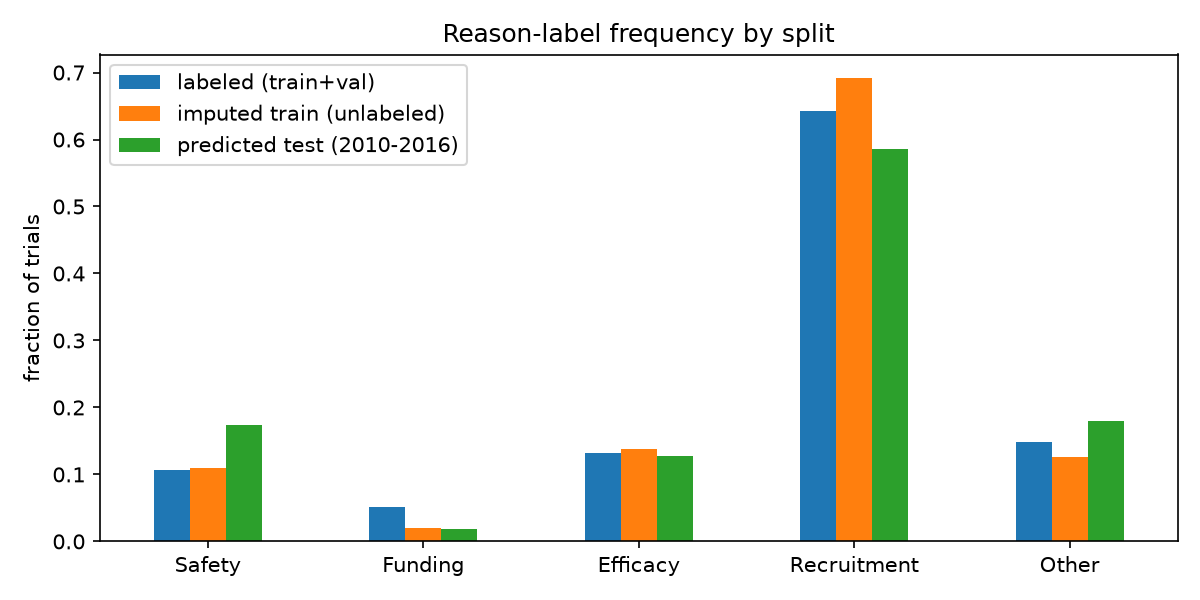
\includegraphics[width=0.95\linewidth]{part1_label_frequency.png}
\caption{Reason-label frequency across the labeled trials, the imputed unlabeled
training trials, and the predicted 2010--2016 test trials.}
\label{fig:p1freq}
\end{figure}

\subsection{Part 2}

Table~\ref{tab:p2val} reports the validation results for each phase. Naive Bayes
ranks trials about as well as logistic regression does, but states its answers far
too confidently, so its log loss of 2.646 is hopeless for a competition scored on
log loss. The stack improves both log loss and PR-AUC in every phase. Adding
recency weights improves log loss further and wins back the F1 that the plain
stack had given up.

\begin{table}[t]
\centering\small
\setlength{\tabcolsep}{3.5pt}
\begin{tabular}{llcccc}
\toprule
Phase & Metric & MNB & Base LR & Stack & $+$Rec \\
\midrule
\multirow{4}{*}{I}
 & F1       & 0.737 & 0.774 & 0.730 & \textbf{0.793} \\
 & ROC-AUC  & 0.717 & 0.780 & 0.772 & \textbf{0.793} \\
 & PR-AUC   & 0.733 & 0.809 & 0.816 & \textbf{0.828} \\
 & log loss & 2.684 & 0.609 & 0.570 & \textbf{0.557} \\
\midrule
\multirow{4}{*}{II}
 & F1       & 0.645 & 0.631 & \textbf{0.661} & 0.648 \\
 & ROC-AUC  & 0.694 & 0.729 & 0.749 & \textbf{0.754} \\
 & PR-AUC   & 0.623 & 0.711 & 0.733 & \textbf{0.735} \\
 & log loss & 2.945 & 0.610 & \textbf{0.591} & 0.593 \\
\midrule
\multirow{4}{*}{III}
 & F1       & 0.796 & 0.813 & 0.817 & \textbf{0.824} \\
 & ROC-AUC  & 0.699 & 0.764 & \textbf{0.787} & \textbf{0.787} \\
 & PR-AUC   & 0.783 & 0.868 & \textbf{0.883} & 0.881 \\
 & log loss & 2.308 & 0.553 & \textbf{0.516} & 0.518 \\
\midrule
\multirow{4}{*}{mean}
 & F1       & 0.726 & 0.739 & 0.736 & \textbf{0.755} \\
 & ROC-AUC  & 0.703 & 0.758 & 0.769 & \textbf{0.778} \\
 & PR-AUC   & 0.713 & 0.796 & 0.810 & \textbf{0.814} \\
 & log loss & 2.646 & 0.591 & 0.559 & \textbf{0.556} \\
\bottomrule
\end{tabular}
\caption{Part~2 validation metrics by phase. Columns are the per-phase
multinomial naive Bayes (MNB), the per-phase criteria-only logistic regression
(Base LR), the stacked ensemble (Stack) and the recency-weighted stack
($+$Rec, $\tau{=}3$). F1 uses a 0.5 threshold; ROC-AUC, PR-AUC and log loss use
predicted probabilities, with $\text{label}=1$ positive. Best value per row in
bold.}
\label{tab:p2val}
\end{table}

The time-ordered holdouts in Table~\ref{tab:p2holdout} ask the question that
matters for the leaderboard: does the ranking still hold when the trials being
scored are later than the trials used to train? It does. Training on everything up
to 2009 and scoring 2010--2013, the stack cuts log loss from 0.5879 to 0.5514, and
recency weighting takes it to 0.5475. On the harder split, training to 2011 and
scoring 2012--2013, the same three steps give 0.5192, then 0.4657, then 0.4553, so
the gap grows as the evaluation moves further from the training years.

\begin{table}[t]
\centering\small
\setlength{\tabcolsep}{3.5pt}
\begin{tabular}{llcccc}
\toprule
Fit cut & Metric & MNB & Base LR & Stack & $+$Rec \\
\midrule
\multirow{4}{*}{$\leq$2009}
 & F1       & 0.8083 & 0.8051 & 0.8090 & \textbf{0.8094} \\
 & ROC-AUC  & 0.6295 & 0.6943 & 0.7248 & \textbf{0.7311} \\
 & PR-AUC   & 0.7301 & 0.7847 & 0.8183 & \textbf{0.8205} \\
 & log loss & 2.4794 & 0.5879 & 0.5514 & \textbf{0.5475} \\
\midrule
\multirow{4}{*}{$\leq$2011}
 & F1       & 0.8576 & 0.8654 & 0.8697 & \textbf{0.8758} \\
 & ROC-AUC  & 0.5970 & 0.7042 & 0.7539 & \textbf{0.7604} \\
 & PR-AUC   & 0.7740 & 0.8290 & 0.8850 & \textbf{0.8865} \\
 & log loss & 2.0120 & 0.5192 & 0.4657 & \textbf{0.4553} \\
\bottomrule
\end{tabular}
\caption{Part~2 time-based holdouts, mean over phases; columns as in
Table~\ref{tab:p2val}. ``Fit cut'' is the last start year in the fitting set: the
2009 cut is evaluated on 2010--2013 and the 2011 cut on 2012--2013. These mimic the later start years of the test set and were used to
select $\tau$. Best value per row in bold.}
\label{tab:p2holdout}
\end{table}

On the Kaggle test set the final submission scores \textbf{0.58688} mean log
loss, against 0.556 on validation---a gap we return to in
Section~\ref{sec:discussion}.

\subsection{Error analysis across reason categories}

Table~\ref{tab:p2errors} and Figure~\ref{fig:p2err} break the failed validation
trials down by phase and stopping reason. Two patterns hold up. First, the
classifier is far more likely to mistake a failed Phase~III trial for a success
(0.57 to 1.00 for the baseline) than a failed Phase~II one (0.00 to 0.38), even
though Phase~III has more training data than Phase~I. Second, the groups large
enough to trust---Phase~II Recruitment with 87 trials, and the three
no-recorded-reason groups with 28, 144 and 82---improve at every step from the
baseline to the stack to the recency-weighted stack. The Phase~I no-reason group
drops from 0.643 to 0.321, less than half its original error rate.

\begin{figure*}[t]
\centering
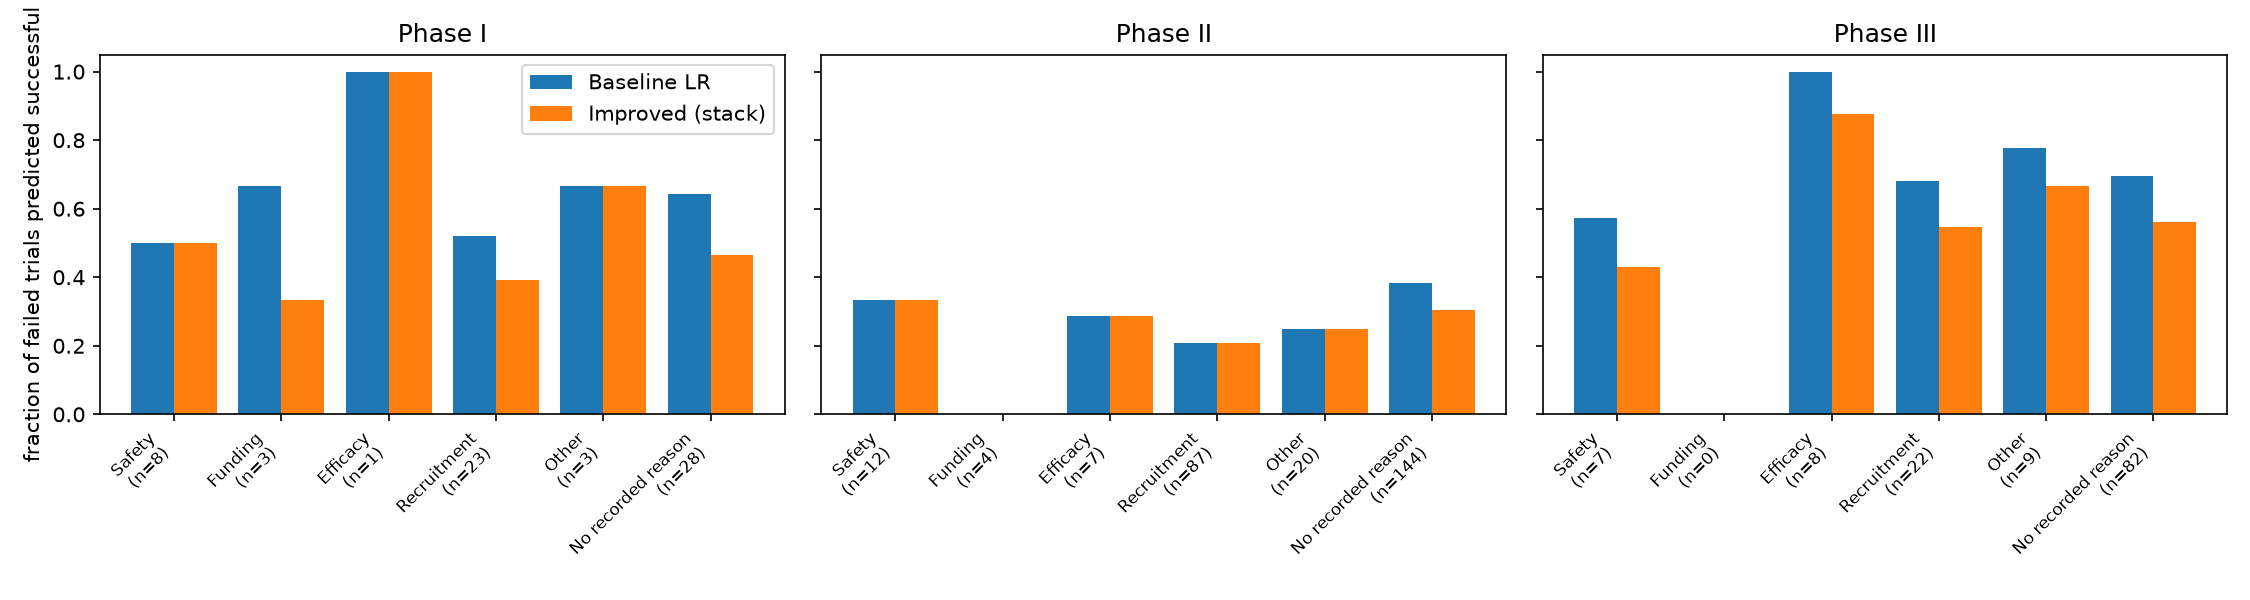
\includegraphics[width=\textwidth]{part2_error_by_reason.png}
\caption{Fraction of failed validation trials incorrectly predicted successful,
by phase and stopping reason, for the criteria-only baseline and the stacked
ensemble. Group sizes are given in the tick labels.}
\label{fig:p2err}
\end{figure*}

\begin{table*}[t]
\centering\small
\begin{tabular}{llccccccc}
\toprule
& & \multicolumn{3}{c}{Group composition} & & \multicolumn{3}{c}{Fraction predicted successful} \\
\cmidrule(lr){3-5}\cmidrule(lr){7-9}
Phase & Reason & $n$ trials & $n$ true & $n$ predicted & & Baseline LR & Improved & Final \\
\midrule
I & Safety             &  8 &  1 &  7 & &  0.500 & 0.500 & 0.375 \\
I & Funding            &  3 &  1 &  2 & &  0.667 & 0.333 & 0.000 \\
I & Efficacy           &  1 &  0 &  1 & &  1.000 & 1.000 & 0.000 \\
I & Recruitment        & 23 &  2 & 21 & &  0.522 & 0.391 & 0.174 \\
I & Other              &  3 &  0 &  3 & &  0.667 & 0.667 & 0.667 \\
I & No recorded reason & 28 &  0 &  0 & &  0.643 & 0.464 & 0.321 \\
\midrule
II & Safety             &  12 &  1 & 11 & & 0.333 & 0.333 & 0.250 \\
II & Funding            &   4 &  1 &  3 & & 0.000 & 0.000 & 0.000 \\
II & Efficacy           &   7 &  0 &  7 & & 0.286 & 0.286 & 0.286 \\
II & Recruitment        &  87 & 12 & 75 & & 0.207 & 0.207 & 0.149 \\
II & Other              &  20 &  3 & 17 & & 0.250 & 0.250 & 0.250 \\
II & No recorded reason & 144 &  0 &  0 & & 0.382 & 0.306 & 0.250 \\
\midrule
III & Safety             &  7 & 1 &  6 & & 0.571 & 0.429 & 0.429 \\
III & Funding            &  0 & 0 &  0 & & ---   & ---   & ---   \\
III & Efficacy           &  8 & 0 &  8 & & 1.000 & 0.875 & 1.000 \\
III & Recruitment        & 22 & 5 & 17 & & 0.682 & 0.545 & 0.455 \\
III & Other              &  9 & 2 &  7 & & 0.778 & 0.667 & 0.556 \\
III & No recorded reason & 82 & 0 &  0 & & 0.695 & 0.561 & 0.585 \\
\bottomrule
\end{tabular}
\caption{Error rates on the 452 failed validation trials, by phase and stopping
reason. ``$n$ true'' counts trials whose reason labels are ground truth from
Part~1; ``$n$ predicted'' counts trials whose reason labels are Part~1 model
predictions. A trial with several reasons appears in each of its reason rows, so
columns do not sum to the phase total.}
\label{tab:p2errors}
\end{table*}

\section{Discussion}
\label{sec:discussion}

\paragraph{Clustering is a poor labeler but a useful prior.}
Used directly, the 30-component mixture is the worst model in
Table~\ref{tab:p1models} (0.780 sample-F1, 0.570 macro-F1). Inspecting the
components explains why: they overwhelmingly separate Recruitment from
everything else, and additional components mostly subdivide Recruitment further
rather than isolating Safety or Efficacy. Since the embeddings do carry that
signal---a purely supervised model reaches Safety F1 0.947---the failure is the
clustering objective, not the features. Unsupervised structure in this space
tracks the dominant topic, and with Recruitment on 64\% of trials the dominant
topic is Recruitment. What does work is demoting the mixture from decision-maker
to prior: as a 0.2-weighted term inside the pseudo-labeling step it raises
cross-validated macro-F1 from 0.805 to 0.814 (and validation sample-F1 from 0.889
to 0.893) over identical self-training without it. The mixture's contribution is
to regularize which unlabeled trials get promoted, not to name their reasons.

\paragraph{Why the extra features fail.}
This is the ablation's most informative result. The reason embeddings are a
compressed encoding of the very stopping-reason text the labels were derived
from, so they are close to a sufficient statistic for the target. Criteria,
disease and drug fields describe \emph{what the trial was}, not \emph{why it
stopped}---a trial can be halted for funding reasons regardless of its indication.
Appending them adds 20--50 parameters per block to a model fit on 157 labeled
trials, so the variance cost arrives immediately while the bias reduction never
does: criteria TF-IDF drops validation sample-F1 from 0.893 to 0.876. The Morgan
fingerprints are the clearest null result, moving cross-validated macro-F1 by
$+0.001$---within repeat-to-repeat noise---which is unsurprising given that 44\%
of trials have no matched drug and receive an all-zero block. \texttt{start\_year}
fails for a more interesting reason: it is genuinely predictive in-sample, because
the labeled trials are deliberately the earliest ones, but the test trials are the
latest, so the model would be extrapolating a year effect fit entirely outside the
test range. Including everything is actively harmful here, not merely redundant.

\paragraph{Rare labels dominate macro-F1.}
Recruitment appears on 64\% of trials and Funding on 5\%. Funding F1 (0.400) and
Other F1 (0.500) rest on 4 and 10 positive validation trials respectively, so a
single trial moves macro-F1 by several points. This is why the validation macro-F1
column in Table~\ref{tab:p1models} is non-monotone with the CV column, and why we
selected on the latter: the final model has slightly lower validation macro-F1
than the balanced LR + $k$NN blend (0.714 vs.\ 0.724) but the best CV macro-F1
(0.814 vs.\ 0.800), and the 235-trial CV estimate is the more reliable of the two.

\paragraph{What the stack buys in Part 2.}
The fitted meta-model weights are informative: criteria LR 0.62, criteria $k$NN
0.55, drug-name LR 0.41, metadata 0.16, with disease (0.06) and ICD (0.03) nearly
ignored and drug-knowledge slightly negative ($-0.11$). The drug-knowledge block
is not useless in isolation---it is redundant once drug names are present, since
targets and pathways are a deterministic function of the matched drug, and the
meta-model subtracts it as a partial correction. The $k$NN's large weight shows
the stack is exploiting near-duplicate trials that the linear criteria model
cannot represent. Pooling phases matters most for Phase~I, which has only 1,012
training rows and gains the most from the shared representation.

\paragraph{The F1 / log-loss trade-off.}
The unweighted stack \emph{lowers} mean validation F1 from 0.739 to 0.736 while
improving log loss (0.591 $\to$ 0.559) and PR-AUC (0.796 $\to$ 0.810). This is not
a regression: F1 at a fixed 0.5 threshold is a statement about calibration near
that threshold, and the stack's meta-model shifts probabilities toward the base
rate, pushing borderline positives below 0.5. Ranking quality, which is what
ROC-AUC and PR-AUC measure, improves in every phase. Recency weighting then raises
the probabilities again and lifts F1 to 0.755, better than either predecessor.
Since the competition metric is log loss, we optimized for calibration and treat
the F1 recovery as a bonus; a project scored on F1 would instead have tuned the
threshold per phase.

\paragraph{Where the errors live.}
The strongest signal in Table~\ref{tab:p2errors} is that failure is hardest to
detect in Phase~III and among trials with no recorded stopping reason. Both follow
from the same cause: these are trials that ran to completion and missed their
endpoint, so nothing in the eligibility text, indication or drug marks them as
different from a successful trial---and Phase~III has a 0.65 success base rate
pulling predictions upward. By contrast, trials stopped for Recruitment or Funding
are administrative failures, and the stack catches them better (Phase~II
Recruitment 0.207 $\to$ 0.149) partly because small, slow-recruiting trials leave
traces in criteria length and drug-count metadata. The improvement is largest
exactly where the baseline was worst: Phase~I no-reason 0.643 $\to$ 0.321,
Phase~III no-reason 0.695 $\to$ 0.585.

\paragraph{How much of the error table to believe.}
Two caveats temper this. Category sizes are small---Safety, Funding, Efficacy and
Other have fewer than 25 failed trials in every phase, and Phase~III Efficacy has
8, so its apparent 1.000 $\to$ 0.875 $\to$ 1.000 trajectory is one trial moving.
Phase~III Funding has no trials at all. More subtly, 171 of the 198 matched reason
labels are Part~1 \emph{predictions} rather than ground truth, and the Part~1
model has roughly 10\% sample-F1 error. Those errors are not random: because the
Part~1 model over-predicts the majority reason, trials are more likely to be
misfiled \emph{into} Recruitment than out of it, which biases the Recruitment row
toward the population average and makes the rare-reason rows noisier than their
sample sizes alone suggest. Only the Phase~II Recruitment row and the three
no-reason rows (whose membership is determined by a join, not a prediction, and so
is error-free) support confident conclusions.

\paragraph{The validation-to-test gap.}
Mean log loss rises from 0.556 on validation to 0.58688 on Kaggle. The cause is
temporal: validation trials started up to 2013 and were split at random from the
training trials, while test trials started 2013--2022, later than every training
row, and the success rate climbs from 0.38 in 2000 to 0.81 in 2013. A model fit on
the pooled base rate is therefore systematically under-confident on test. Recency
weighting is our response and was the single largest holdout gain we found
(0.5514 $\to$ 0.5475 fitting to 2009; 0.4657 $\to$ 0.4553 fitting to 2011); it
redistributes mean test predictions per phase rather than inflating them
uniformly---Phase~III rises from 0.711 to 0.738 while Phase~I falls from 0.617 to
0.598 and Phase~II from 0.565 to 0.557---because recent Phase~III trials succeeded
far more often than recent early-phase ones. The residual gap reflects what we deliberately did not model. We
built an alternative submission that lets the meta-model learn an explicit
Phase~III year trend (Phase~III success rises 0.71 in 2009 to 0.96 in 2013), which
pushes mean Phase~III test predictions to 0.788; on the holdouts it gains only
about 0.001 log loss, and it extrapolates a trend fit on four years out to 2022,
so we kept it as a recorded alternative rather than the submission. A per-phase
trend for all phases was rejected outright: it fits flat or negative Phase~I/II
slopes and would drive those predictions below the training base rate. Beyond the
year effect, the test trials differ in disease and drug mix, and no amount of
reweighting on pre-2014 data can calibrate for that.


{
    \small
    \bibliographystyle{ieeenat_fullname}
    \bibliography{main}
}

\end{document}
